\chapter{Các phần cứng và sơ đồ được dùng trong đề tài} \label{phancung-sodo}
%\section*{Các phần cứng} \label{phuluc-phancung}
\subparagraph{Các phần cứng dùng điều khiển chính}{~\\}
\begin{figure}[!h]
\begin{center}
	\subfloat[PIC 16F887 \label{Fig:HW_16F887}]
		{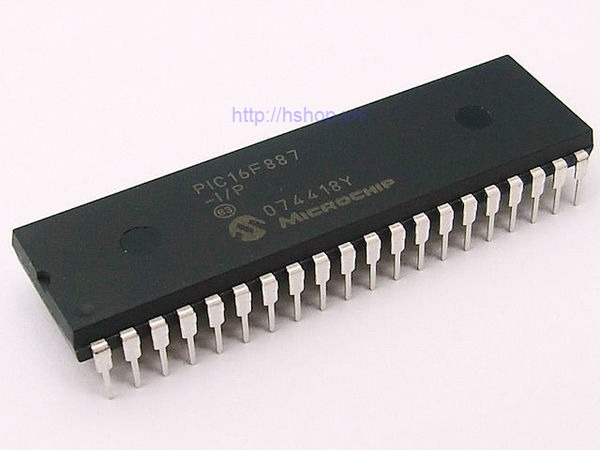
\includegraphics[scale=.2]{HW_16F887}}
	\hspace{.5cm}	
	\subfloat[Mạch nạp PICKIT2 K150\label{Fig:HW_PICKIT}]%, hỗ trợ các dòng PIC: $10$, $12$, $12F$, $16C$, $16F$, $18F$
		{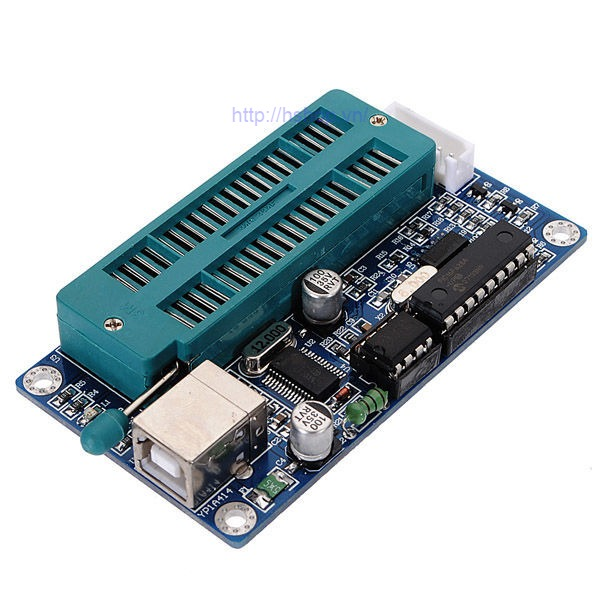
\includegraphics[scale=.15]{HW_PICKIT}}
	\hspace{.5cm}	
	\subfloat[Cảm biến nhiệt độ DS18B20\label{DS18B200}]
		{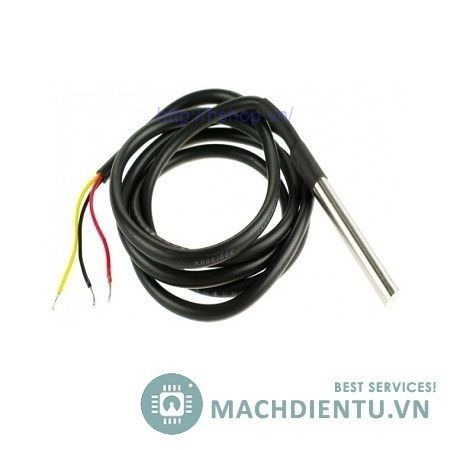
\includegraphics[scale=.2]{HW_DS18B20} }\\
	\subfloat[LCD 16x2\label{LCD1602}]
		{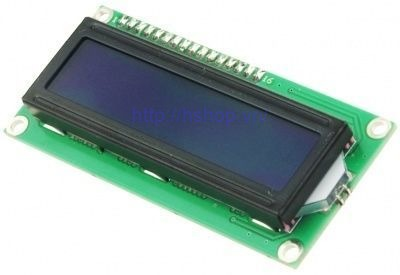
\includegraphics[scale=.3]{HW_LCD1602}}
	\hspace{.5cm}
	\subfloat[Relay 5VDC với Opto cách ly\label{RELAY}]
		{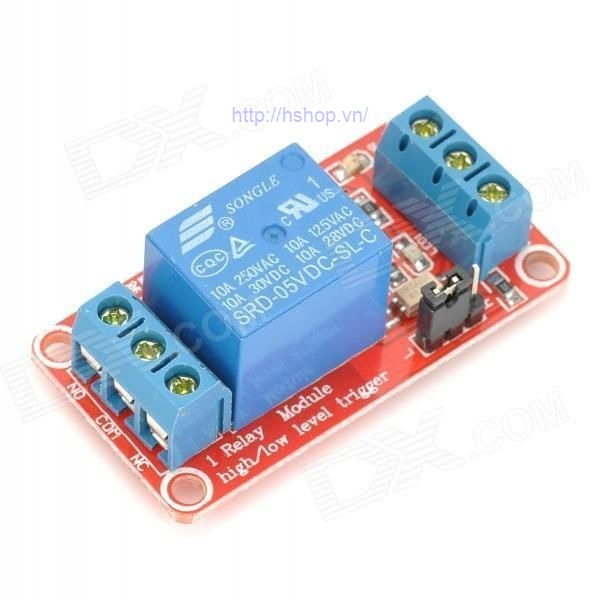
\includegraphics[scale=.15]{HW_RELAY}}
	\hspace{.5cm}	
	\subfloat[Động cơ 5VDC]
		{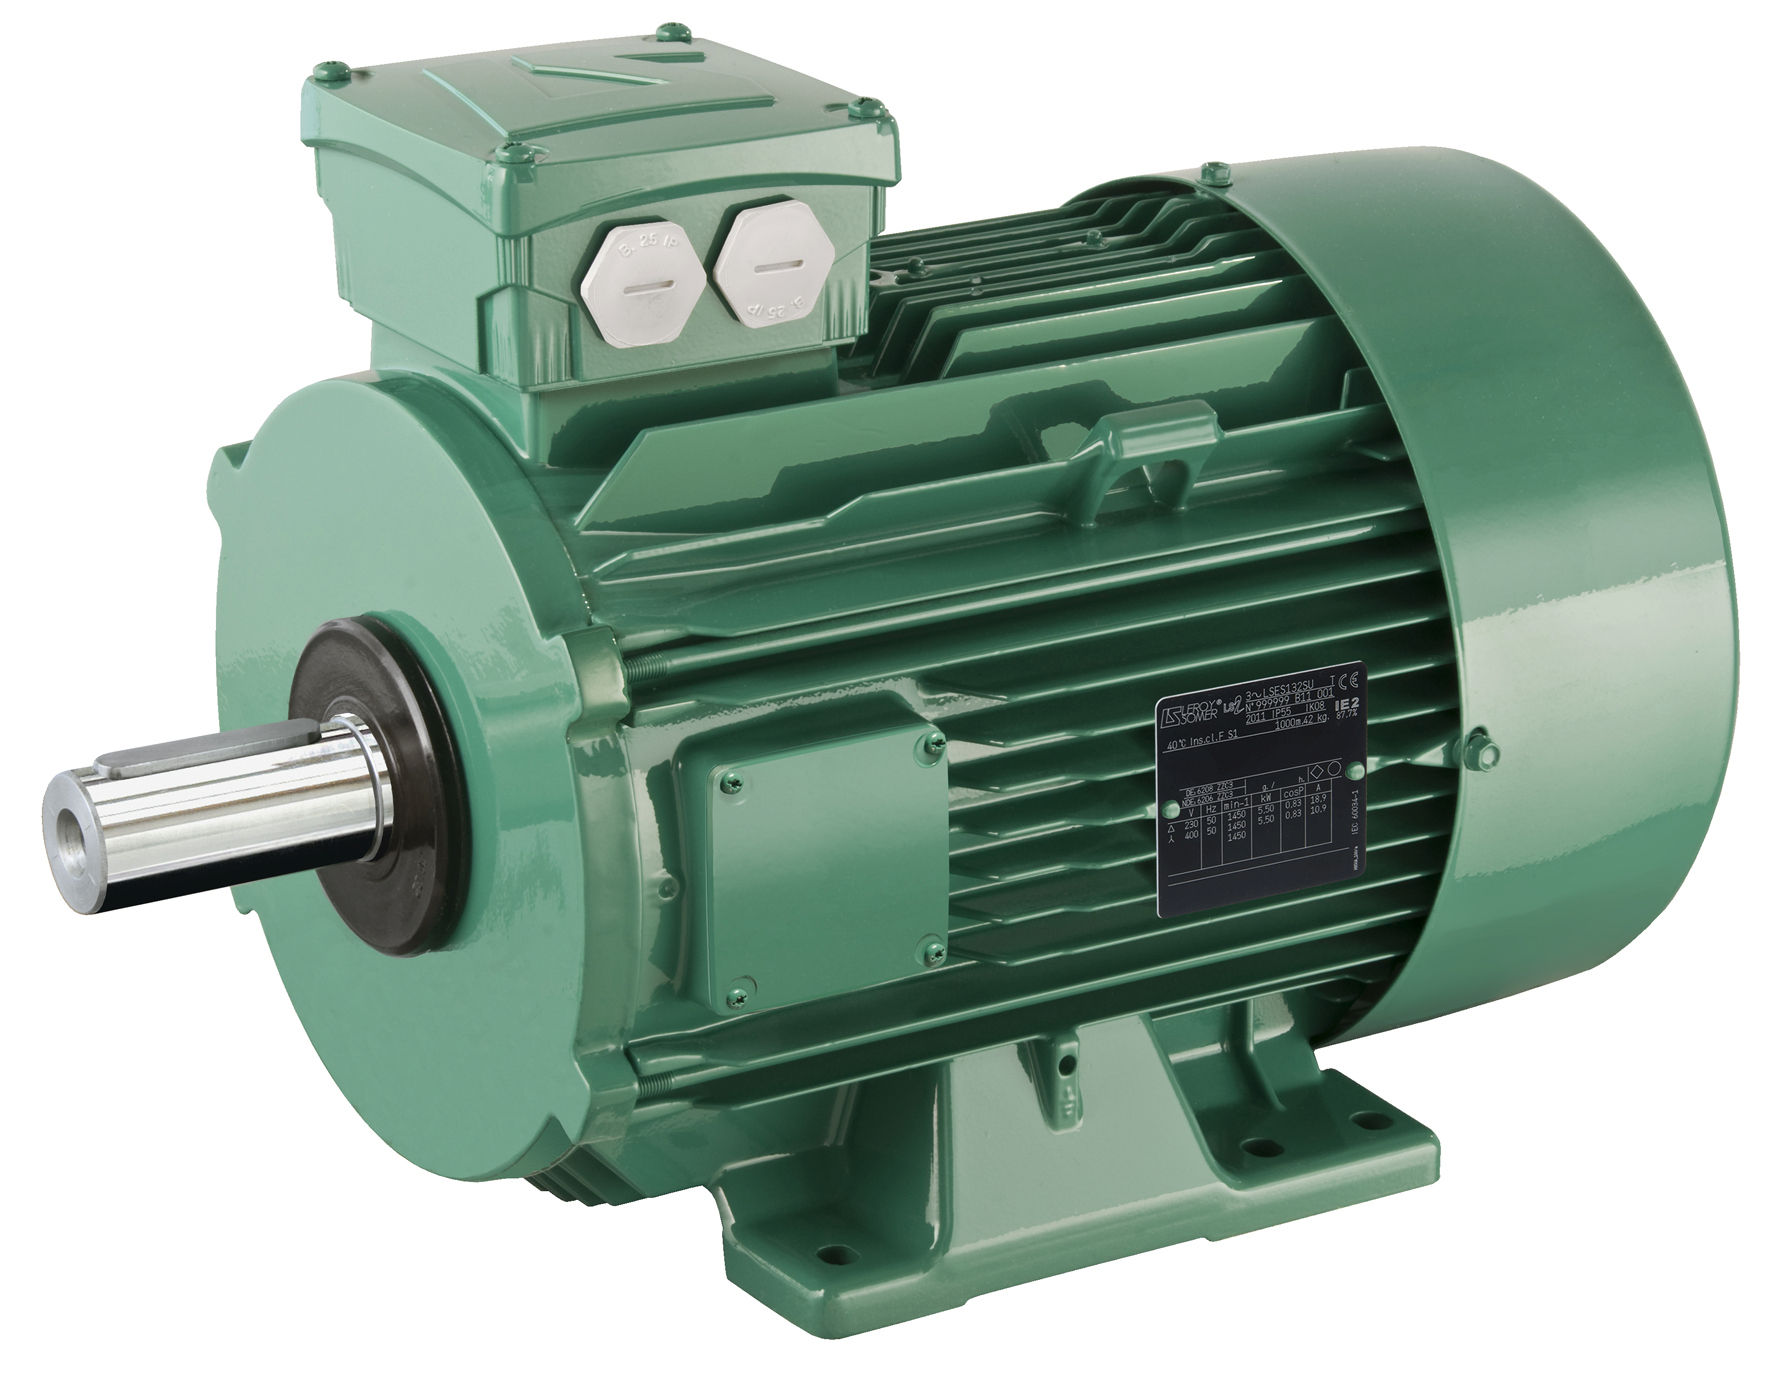
\includegraphics[scale=.3]{Motor}}\\
	\subfloat[Nút nhấn loại 4 chân]
		{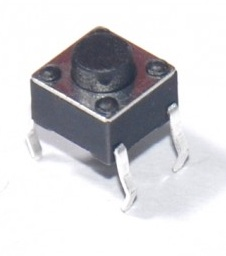
\includegraphics[scale=.4]{HW_BUTTON}}
	\hspace{.5cm}	
	\subfloat[Biến trở $10k\Omega$]
		{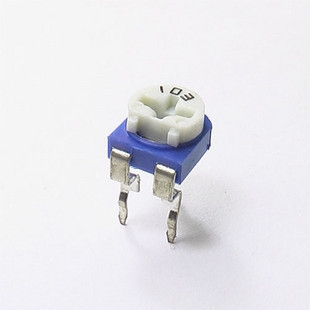
\includegraphics[scale=.3]{VAR_10k}}
\end{center}
\caption{Các phần cứng chính dùng điều khiển cho mô hình}
\end{figure}
\subparagraph{Các linh kiện hỗ trợ và phụ kiện kết nối}{~\\}

\begin{figure}[!h]
\begin{center}
\subfloat[Điện trở $4.7k\Omega$]
	{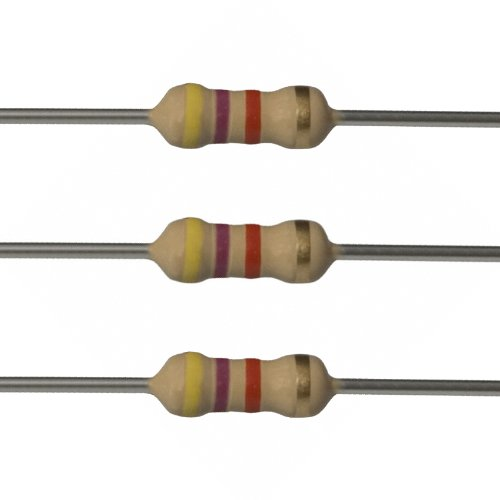
\includegraphics[scale=.2]{RES4k7}}
\hspace{.5cm}
\subfloat[Thạch anh tần số $20MHz$]
	{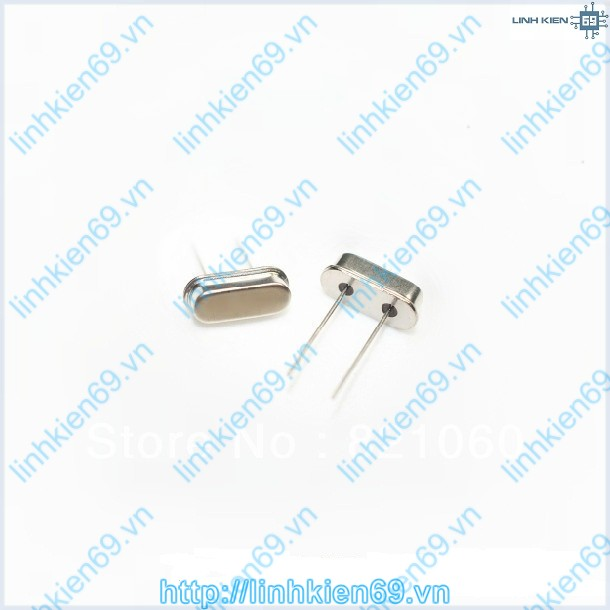
\includegraphics[scale=.15]{THACH_ANH}}
\hspace{.5cm}
\subfloat[Tụ điện $15pF$]
	{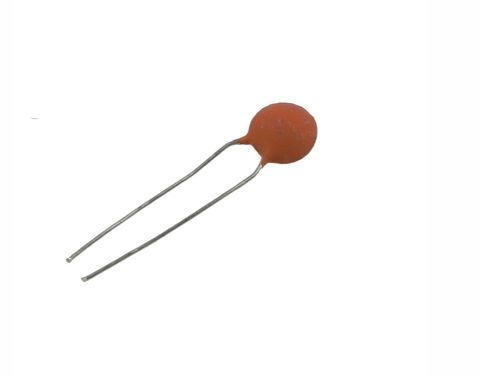
\includegraphics[scale=.8]{CAP}}\\
\subfloat[Domino đấu nối]
	{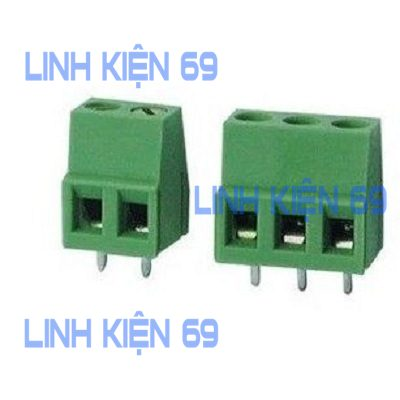
\includegraphics[scale=.4]{HW_DOMINO}}
\hspace{.5cm}
\subfloat[Đế IC 40 chân]
	{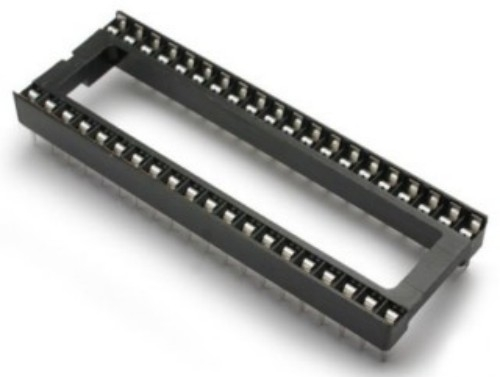
\includegraphics[scale=.3]{HW_DE_IC}}
\hspace{.5cm}
\subfloat[Rào cái loại đơn]
	{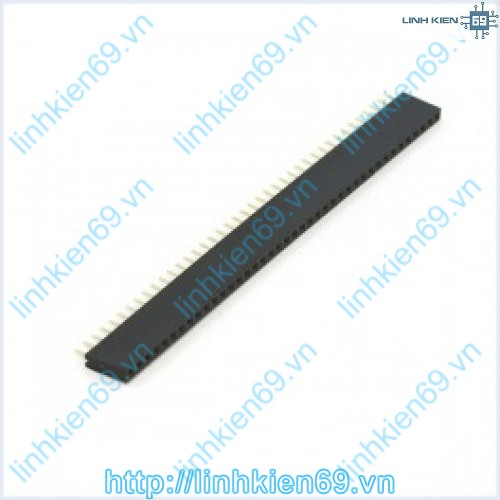
\includegraphics[scale=.25]{RAO_CAI}}\\
\subfloat[Rào cái loại đơn]
	{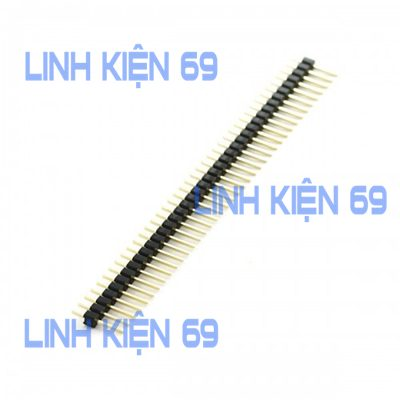
\includegraphics[scale=.35]{RAO_DUC}}
\hspace{.5cm}
\subfloat[Dây kết nối 2 đầu cái - cái]
	{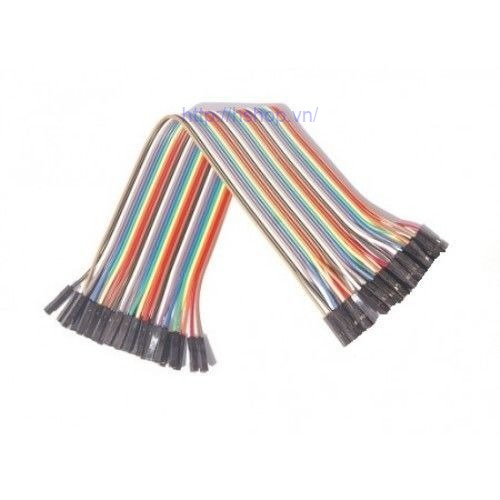
\includegraphics[scale=.3]{WIRE}}
\hspace{.5cm}
\subfloat[Testboard hàn mạch]
	{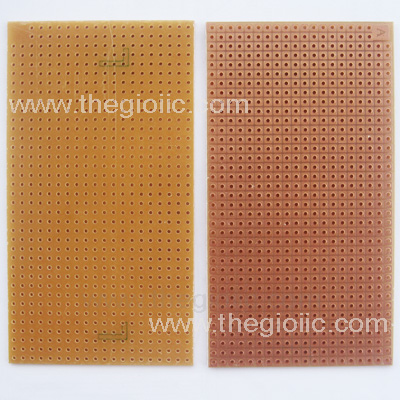
\includegraphics[scale=3]{TB_HAN}}
\end{center}
\end{figure}
\subparagraph{Các phụ kiện khác}
\begin{list}{--}{}
\item \textit{Bộ nguồn cấp cho vi điều khiển}: nguồn $5VDC - 2A$.
\item Các dụng cụ thực hành điện tử: VOM, mỏ hàn, chì hàn, kiềm, dây kết nối khi hàn, \ldots
\end{list}